\documentclass[tikz,border=7pt]{standalone}
% end preamble
\usepackage[e]{esvect}
\usetikzlibrary{calc, angles}
\tikzset{
  half line/.style = {
    shorten >=-21mm, -latex
  },
  vector/.style = {
    thick,-latex
  },
  dot/.style = {
    insert path={
      node[scale=2]{.}
    }
  }
}
\begin{document}
  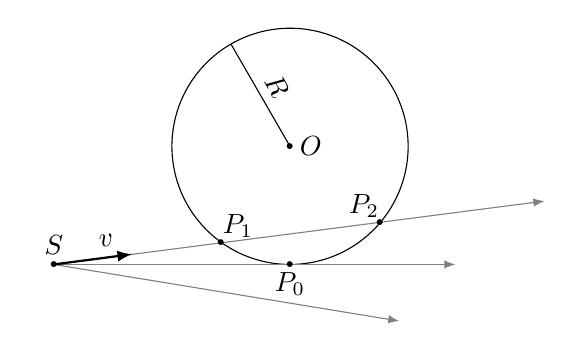
\begin{tikzpicture}
    % les coordonées des points
    \path
      (0,0) coordinate (O)
      (120:1.5) coordinate (R)
      (-3,-1.5) coordinate (S)
      (0,-1.5) coordinate (P0)
      (-40:1.5) coordinate (P2)
      (-125.5:1.5) coordinate (P1) % à la main
      (-110:2) coordinate (U)
      ($(S)!1cm!(P1)$) coordinate (v)

      (3.1,-2.1) coordinate (phantom)
    ;
    % le cercle
    \draw
      (O) circle(1.5)
    ;
    % les rayons
    \draw[gray]
      (S) edge[half line] (P0)
      (S) edge[half line] (P2)
      (S) edge[half line] (U)
      (S) edge[vector, black] node[above, sloped, pos=.7]{$\vv{v}$} (v)
    ;
    % les points
    \path
      (O) [dot] node[right]{$O$}
      (S) [dot] node[above]{$S$}
      (P0) [dot] node[below, circle, inner sep=0pt]{$P_{0}$}
      (P1) [dot] node[above right, circle, inner sep=1pt]{$P_{1}$}
      (P2) [dot] node[above left, circle, inner sep=1pt]{$P_{2}$}
      (O) edge node[sloped, above]{$R$} (R)
    ;
  \end{tikzpicture}
\end{document}
